\documentclass[final]{beamer}
\usepackage[size=a1,orientation=portrait,scale=1.25]{beamerposter}

% Theme colors
\definecolor{myblue}{RGB}{2,62,138}
\definecolor{lightbluebg}{RGB}{230,240,255}

% Additional packages for background image
\usepackage{tikz}
\usepackage[overlay,absolute]{textpos}

% Beamer style adjustments
\usetheme{default}
\usecolortheme{default}
\setbeamercolor{block title}{fg=white,bg=myblue}
\setbeamercolor{block body}{fg=black,bg=lightbluebg}
\setbeamercolor{item}{fg=myblue}
\setbeamercolor{title in headline}{fg=white,bg=myblue}
\setbeamercolor{author in headline}{fg=white,bg=myblue}
\setbeamercolor{date in headline}{fg=white,bg=myblue}
\setbeamercolor{footline}{bg=myblue, fg=white}
\setbeamertemplate{itemize items}[circle]
\setbeamertemplate{footline}{
  \leavevmode\hbox{
    \begin{beamercolorbox}[wd=\paperwidth,ht=4ex,dp=1ex,center]{footline}
	\normalsize
    \textbf{EdMedia 2025, Barcelona, May 19--23}\hfill
    \texttt{rw86221@stud.uws.edu.pl, dariusz.mikulowski@uws.edu.pl }
    \end{beamercolorbox}}
}
% Title and authors with logos
\title{\centering\huge\textbf{Developing The Imagination and Logical Thinking of Visually Impaired Pupils Through Sound-Based Puzzles and Riddles}}

\author{\Large\textbf{Rafal Wilinski$^1$ and Dariusz Mikulowski$^1$}} 
\institute{\Large$^1$University of Siedlce, Faculty of Exact and Natural Sciences}
\date{}

\newcommand{\imgsize}{.95\textwidth}
\newcommand{\rimgsize}{.92\textwidth}

\begin{document}

\begin{frame}[t]

\begin{tikzpicture}[remember picture, overlay]
  \node[anchor=center] at (current page.center) {
    
\includegraphics[width=\paperwidth,height=\paperheight]{img/tlo.png}
  };
\end{tikzpicture}
\titlepage

\vspace{-2cm}

\begin{columns}[t,totalwidth=\textwidth]

\begin{column}{0.49\textwidth}

\begin{block}{Motivation and Background}
Logic games like puzzles and riddles are very popular among users. However, blind people have limited access to this type of entertainment due to a lack of accessibility. 

The project aimed to create a universal application that develops the logical thinking and imagination of visually impaired students through interactive riddles and audio-supported puzzles. The application enables joint play for sighted and blind people, thus supporting the integration and development of their cognitive competencies.
\end{block}

\begin{block}{Related Works} 
Numerous studies have confirmed the positive impact of educational games on developing cognitive skills and creativity.

(Barnabé et al. 2023) demonstrated that system dynamics-based games can significantly enhance learners' critical thinking and project management competencies.

Similarly, (Mercier et al. 2024) found that frequent engagement with board games correlates with higher workplace creativity and a stronger creative self-concept. 

In another study, (Chukusol et al. 2024) introduced a challenge-based hybrid learning model using virtual board games, which proved effective in fostering research creativity and critical thinking among students.

For visually impaired users, platforms like \textbf{RS Games} and \textbf{Crazy Party Games}, (Pragma, n.d.) offer sound-based games without graphical user interfaces, focusing solely on audio navigation. 

Although accessible for blind users, these games often exclude sighted users who might wish to play collaboratively. 

As (Lewis n.d.) highlights, many audio games lack a GUI, making them less inclusive. 

In contrast, the application presented in our work (Wilinski R. 2025) combines a sound interface with a universally designed graphical layout, enabling joint gameplay and learning experiences for blind, visually impaired, and sighted users. 
\end{block}

\begin{block}{Audio Puzzle Game - How it Works?} 
A game was implemented as a web application in Angular with a database in Google Cloud.

It was created in accordance with the ARIA standard.
Due to this, it is fully compatible with screen readers. 

\begin{center}
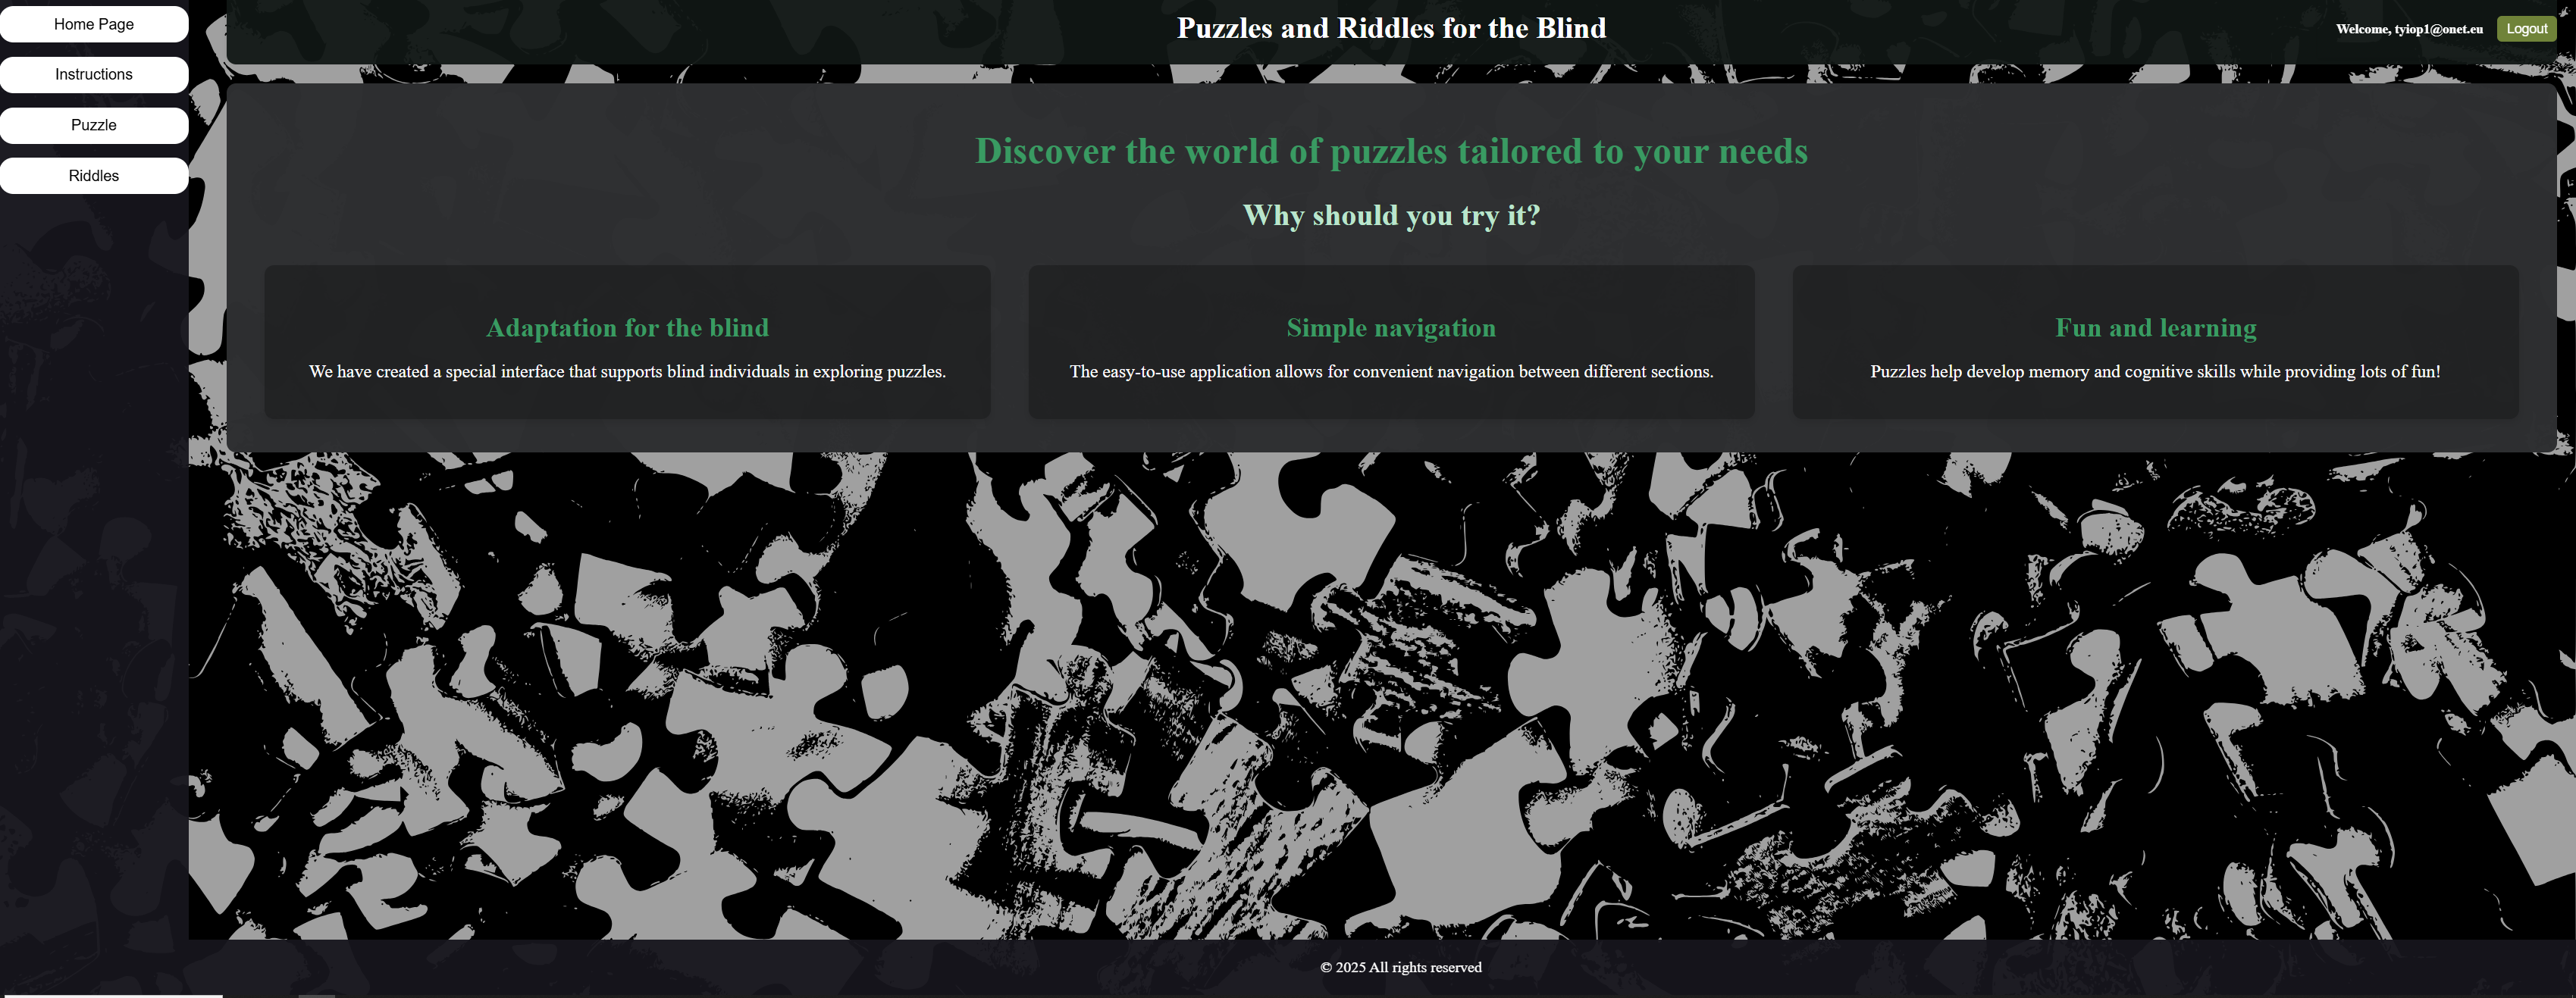
\includegraphics[width=\imgsize]{img/mainpage.png}

Figure 1: Main screen of the puzzle game.
\end{center}
\vspace{0.5cm}

The game consists of two modules.

The first one is the \textbf {riddle solving} module where  the user can solve logical text riddles that have been grouped into several sets.

\begin{center}
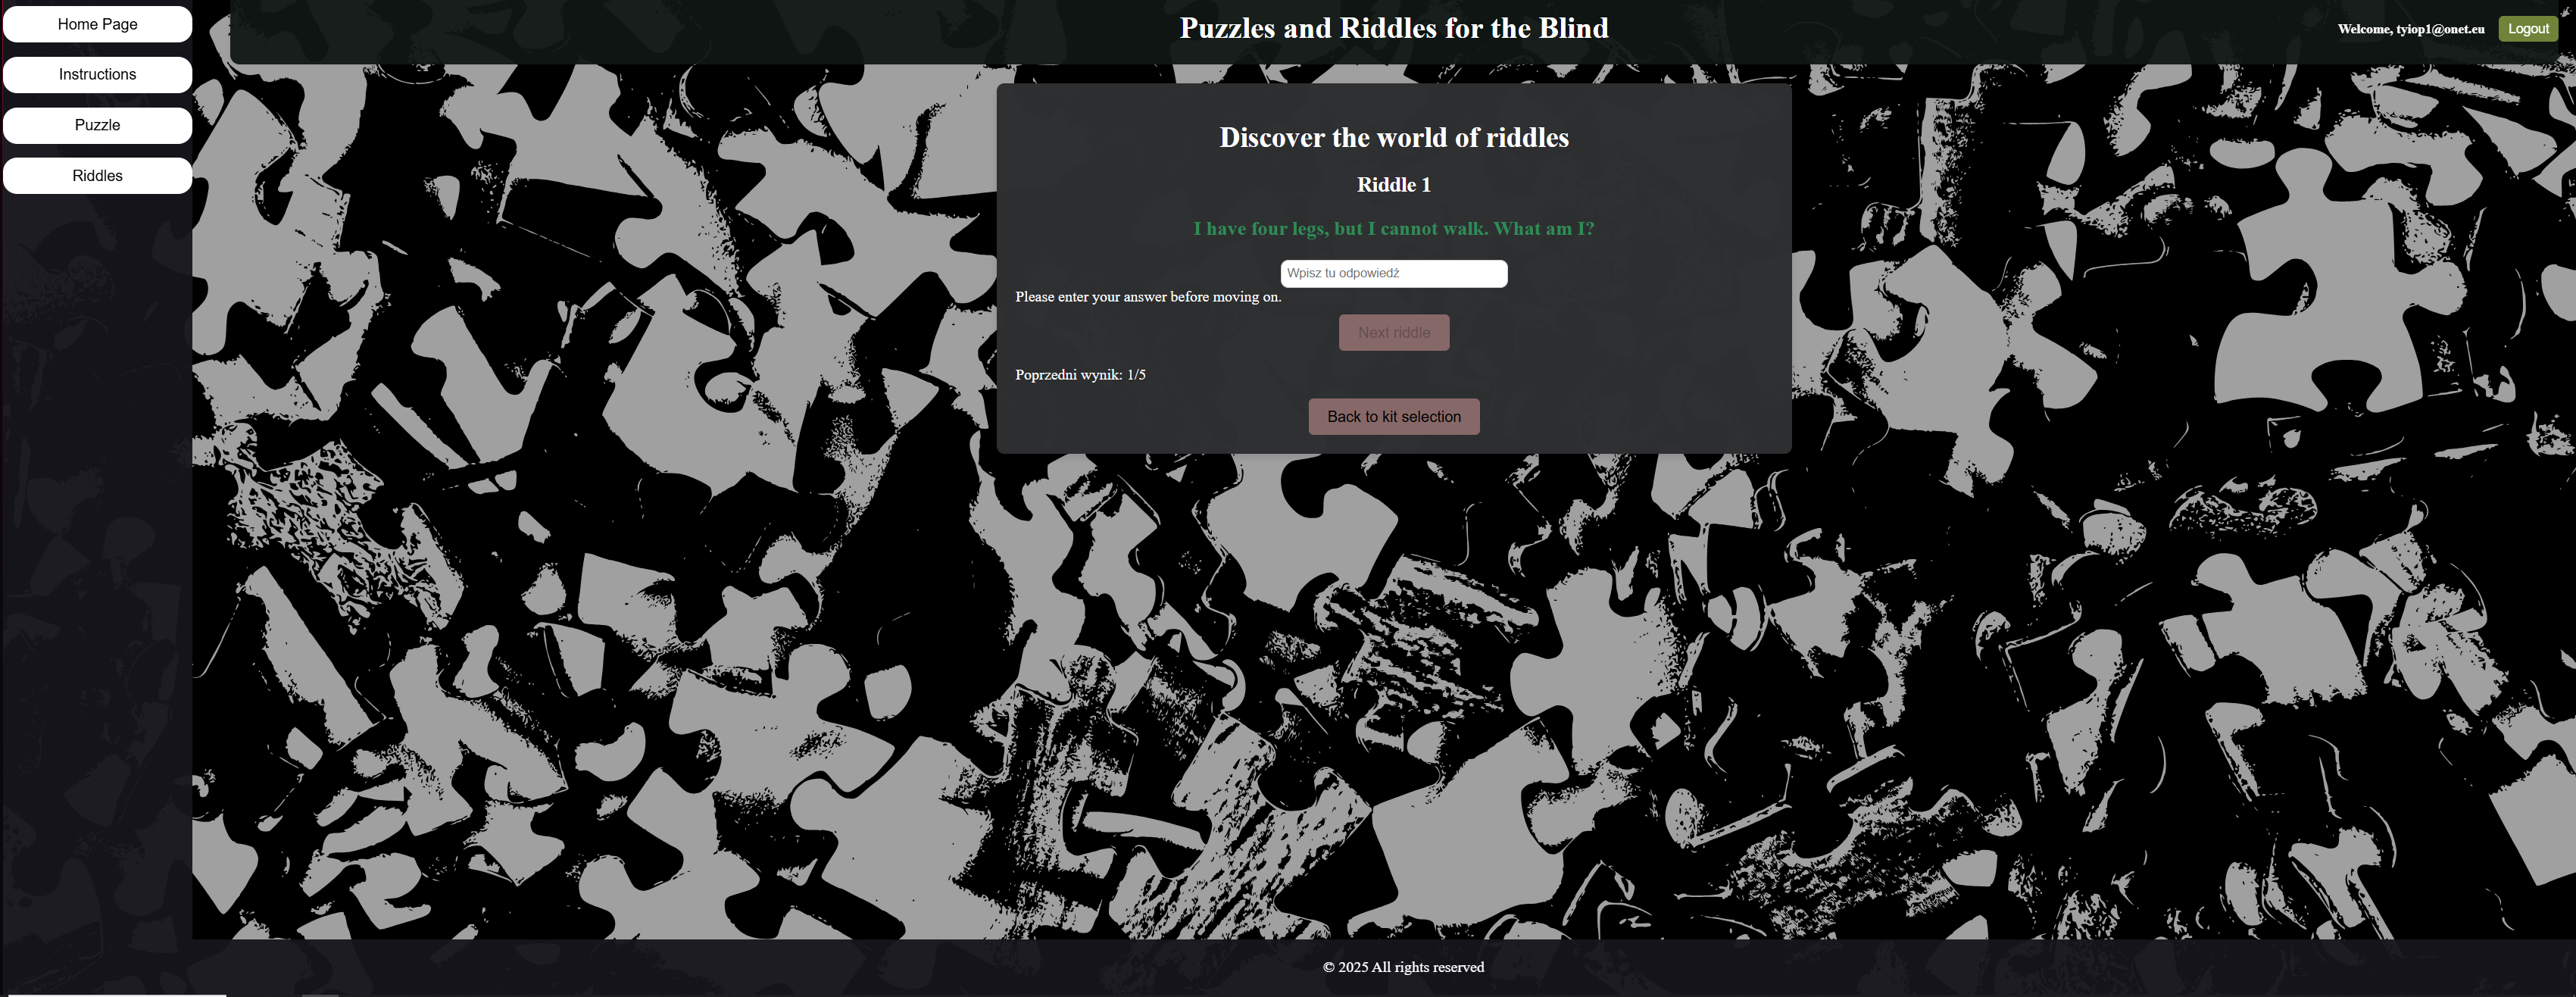
\includegraphics[width=\imgsize]{img/riddles-middle.png}

Figure 2: Solving riddles 
\end{center}

After solving the whole set of riddles, the player is notified of the result of his fun.

\begin{center} 
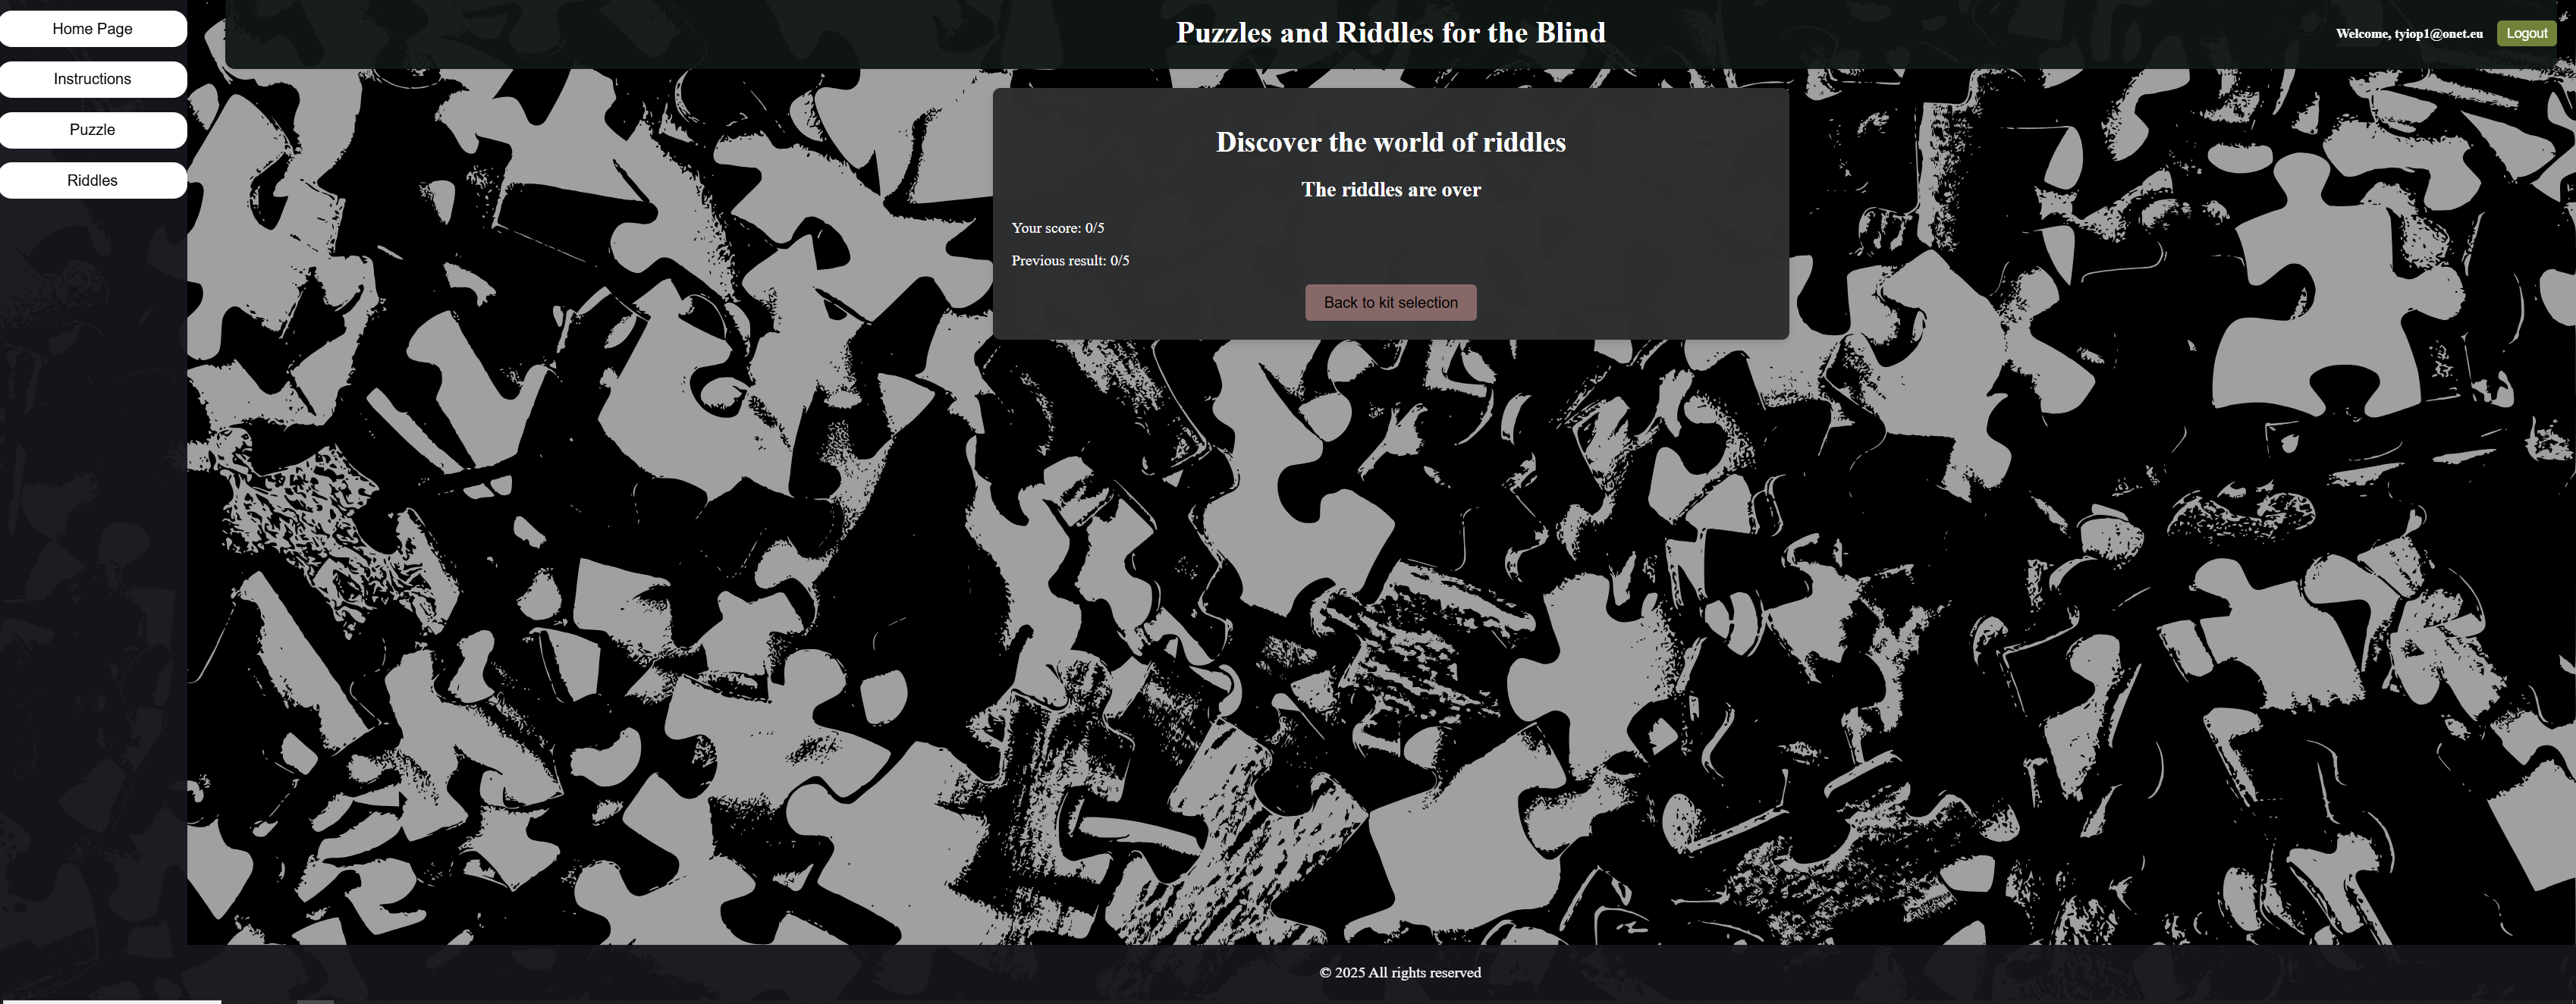
\includegraphics[width=\imgsize]{img/riddles-end.png}

Figure 3: Results of riddle game 
\end{center}
\end{block}
\end{column}

\begin{column}{0.49\textwidth}  % ------------------------------------------

\begin{block}{Audio Puzzle Game }

The next one is an \textbf {audio puzzle solving} module.
The user can choose one of several sets of puzzles that are grouped according to the level of difficulty.

The easiest level is one in which the user receives a description and an indication of place where he should arrange each piece.

\textit{E.g, a shadow of a tree and a meadow. Put it  on lower right corner.}

More difficult levels have no descriptions about their correct place in the puzzle.

\begin{center} 
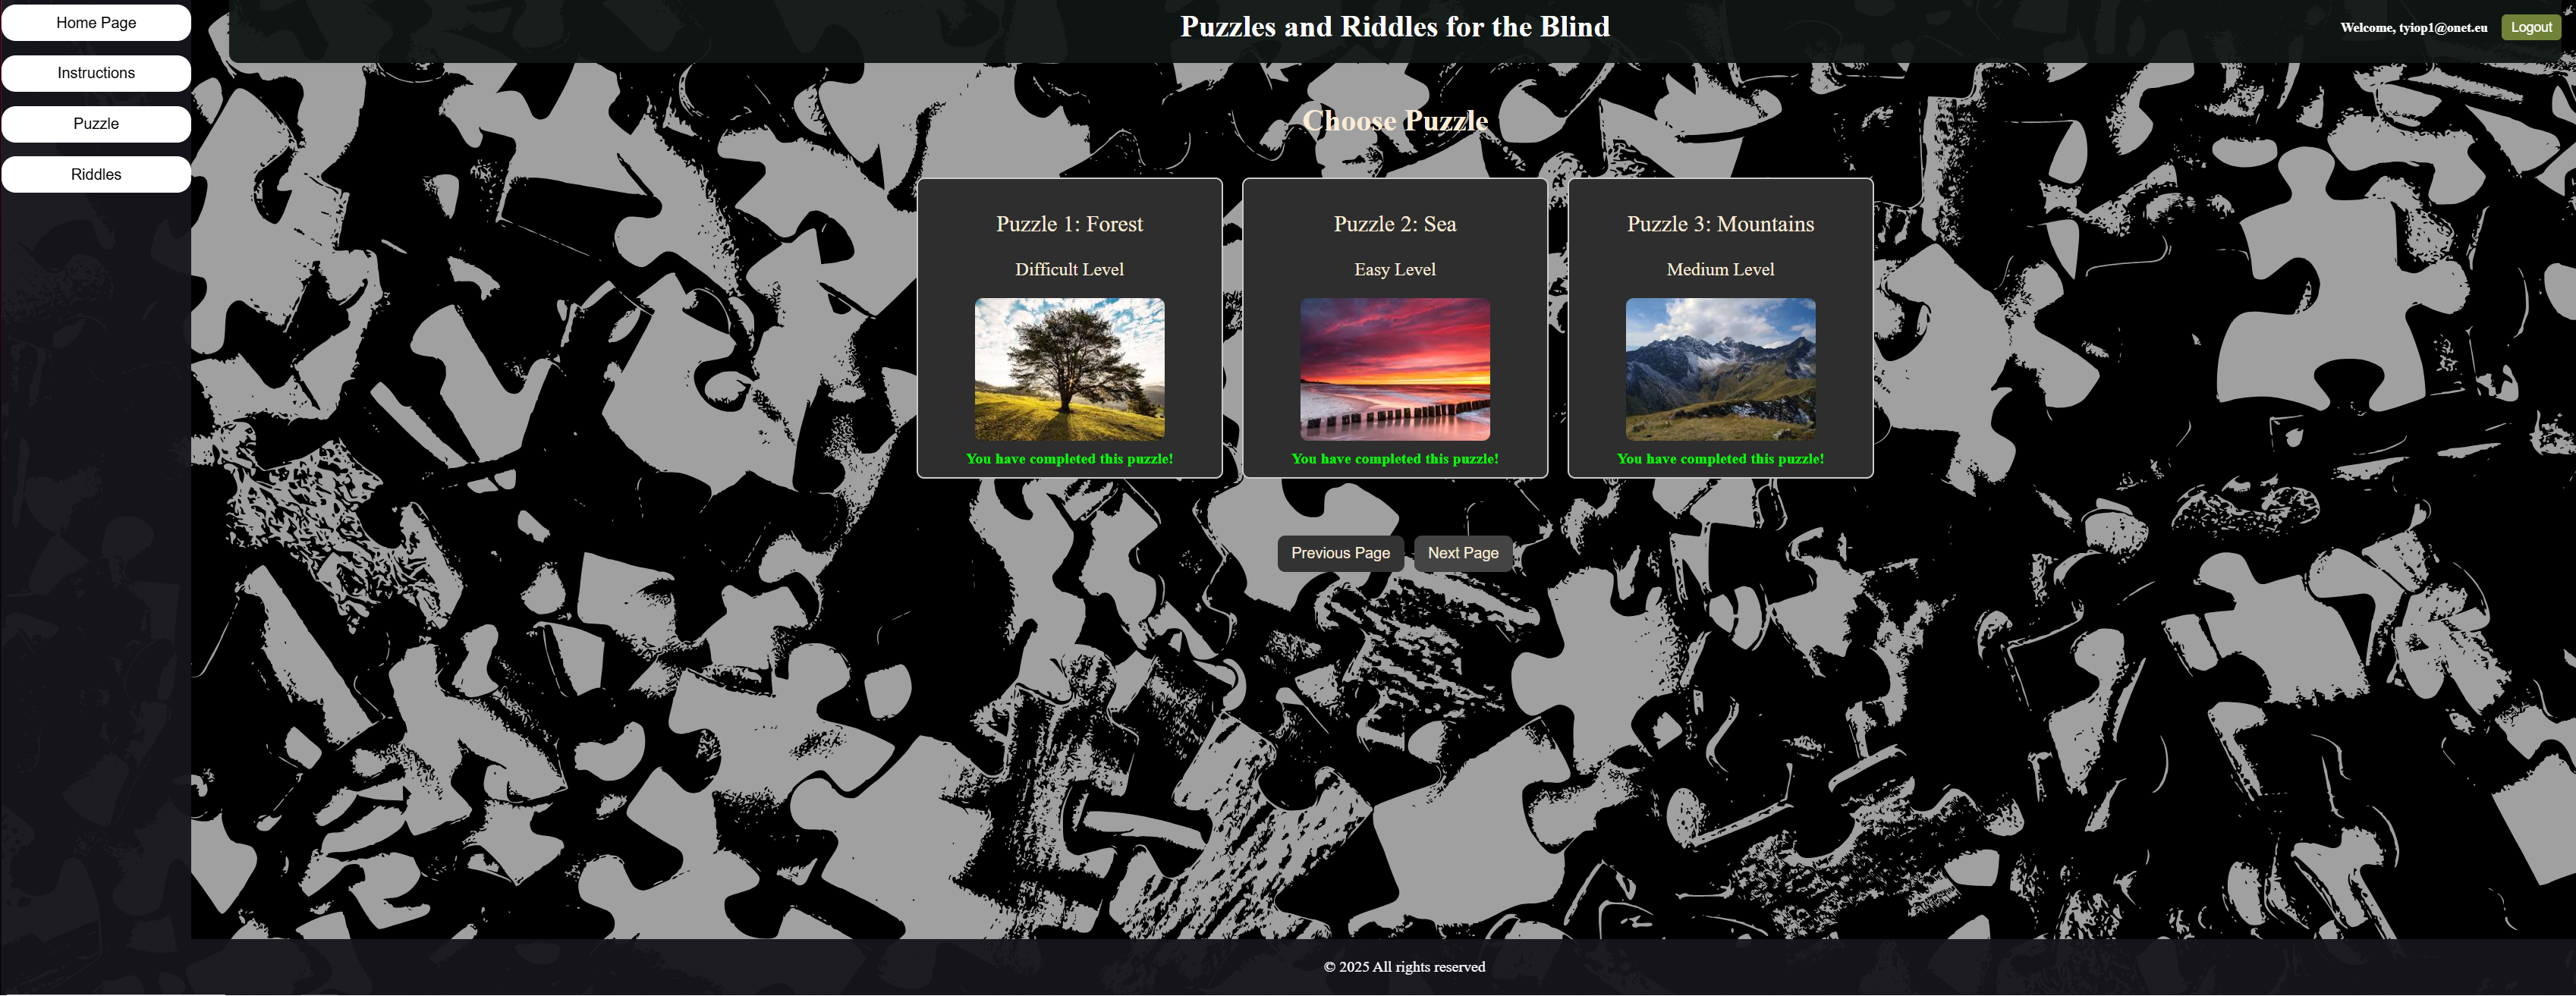
\includegraphics[width=\rimgsize]{img/Puzzle-mainscreen.png}

Figure 4: Selecting puzzle to solve
\end{center}

While solving the puzzle, the player moves around the board using the arrow keys and replaces pieces of puzzles with the enter key.

The descriptions help in the arrangement of elements and their view  are read on a regular basis.

\begin{center}
		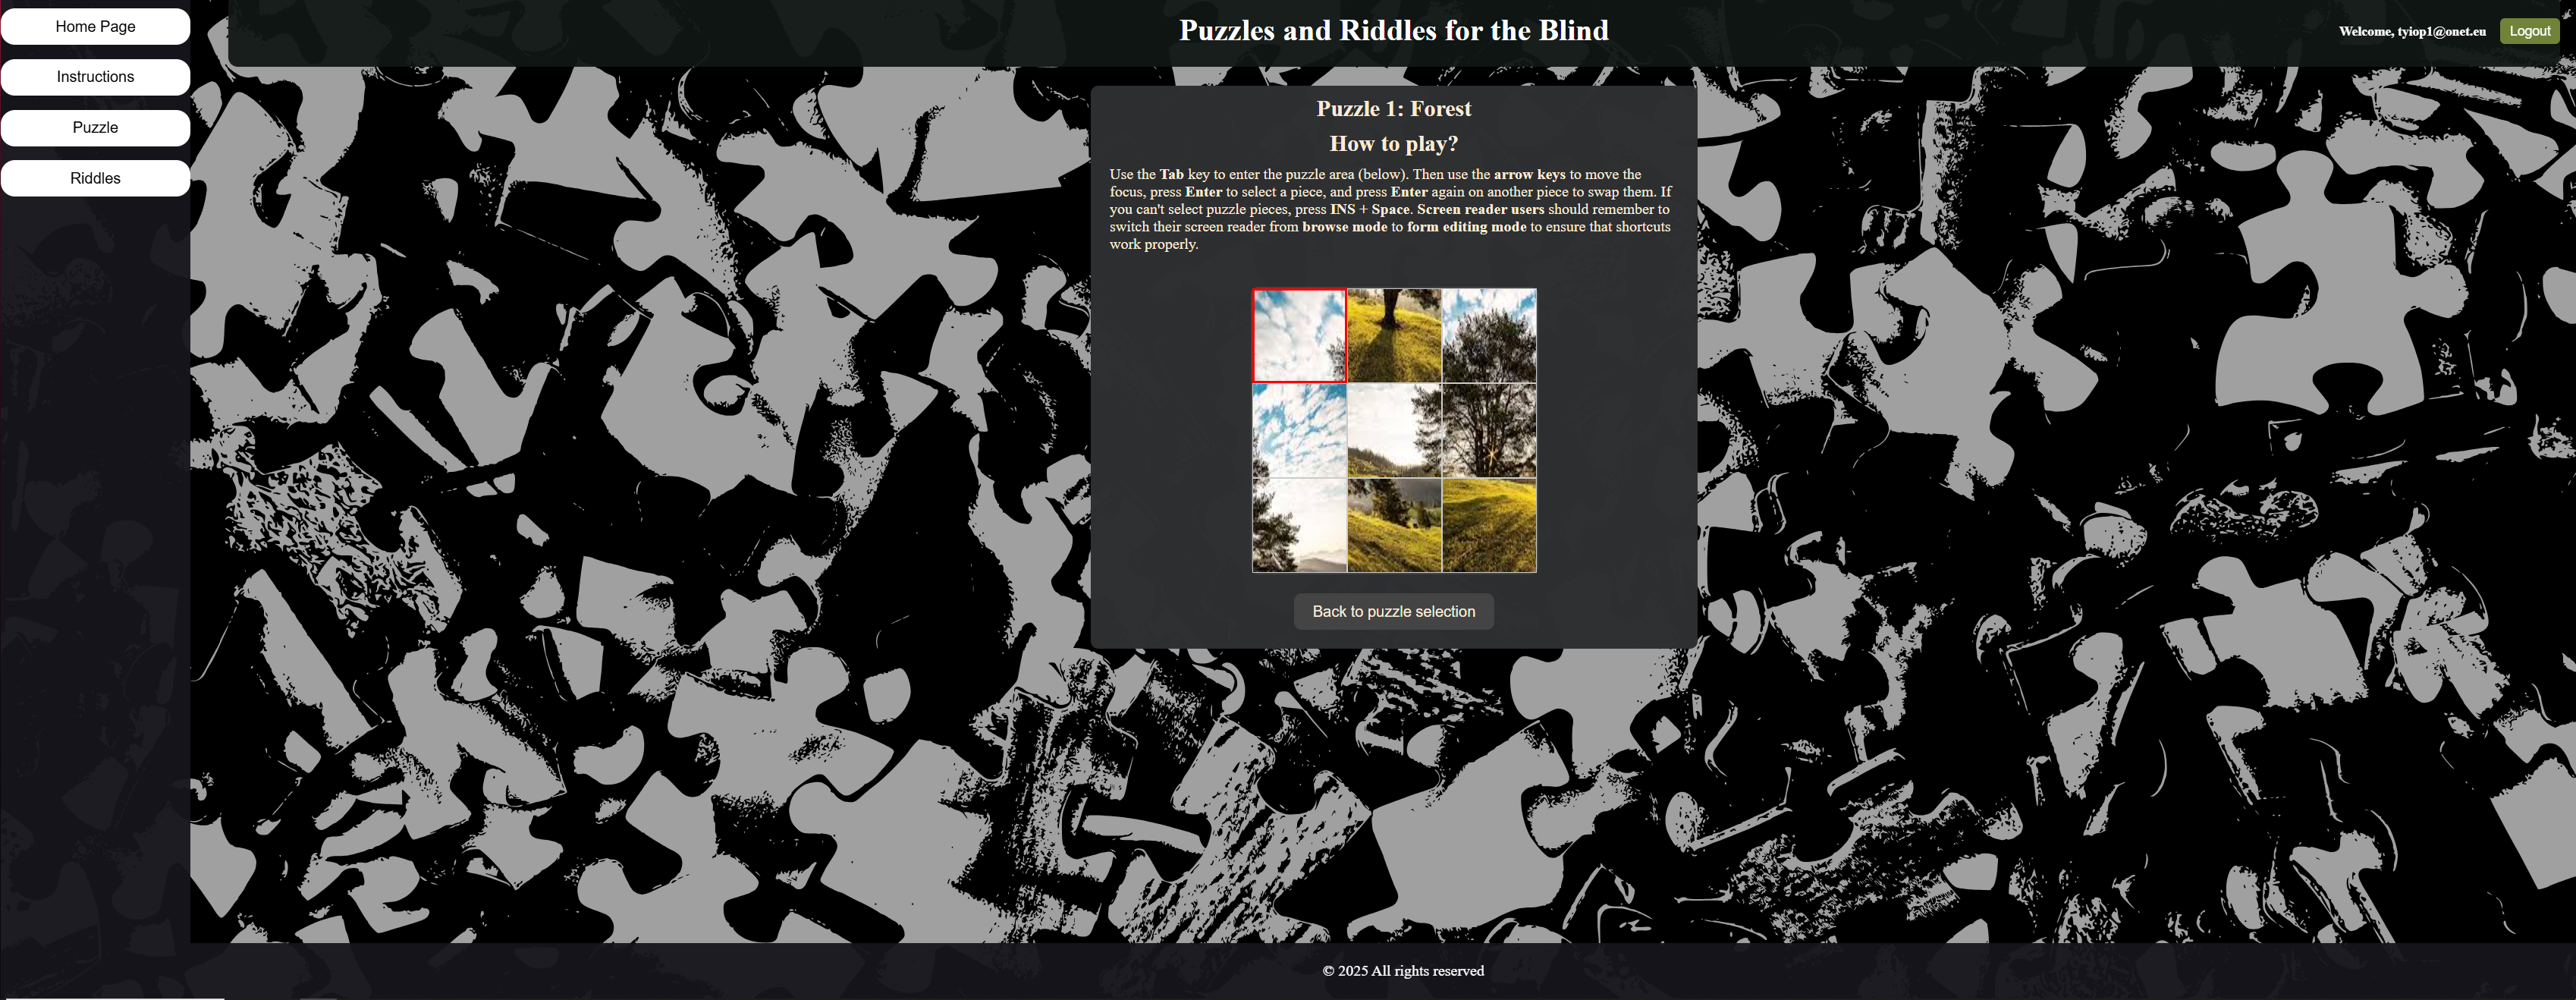
\includegraphics[width=\rimgsize]{img/puzzle-solving-forest.png}

Figure 5: Solving the puzzle with forest picture, with audio description. 
\end{center}

After solving the puzzle, the result is presented to the user.

\begin{center}  
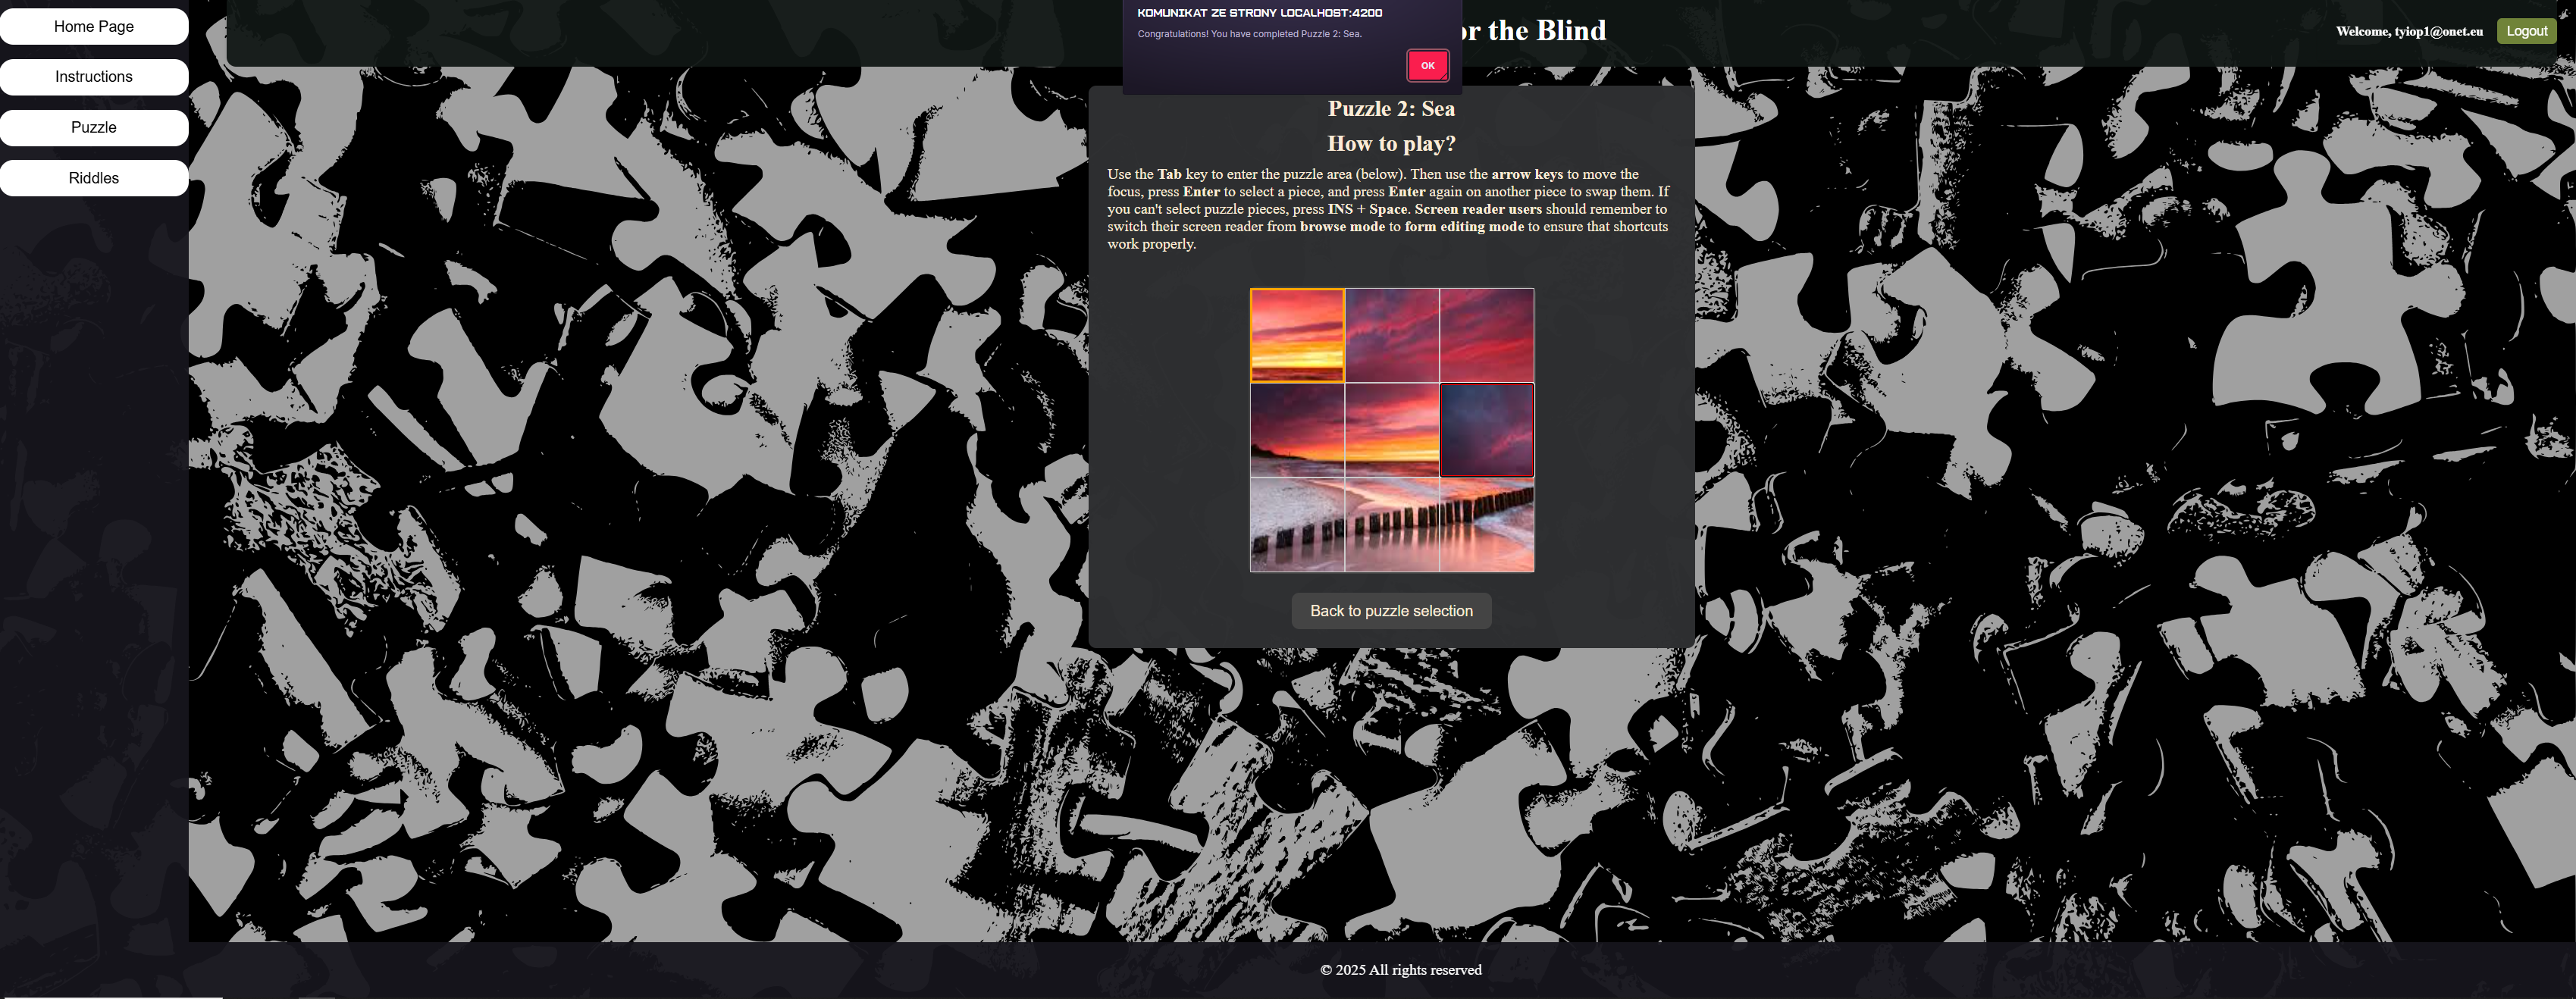
\includegraphics[width=\rimgsize]{img/puzzle-end.png}

Figure 6: Results of solved puzzles
\end{center}
\end{block}

\begin{block}{Results}
The pilot version of the game has been tested by three blind users. 

A positive reception was obtained, especially for the feature of description of the puzzle elements and intuitive navigation across the puzzle game. 

Users have reported a desire to expand the application with new sets of puzzles and the ability to add their puzzles after logging in.

The modernization and development of the application are planned in these directions.
\end{block}

\begin{block}{Conclusions}
The proposed solution is an example of an inclusive approach to educational games, combining a graphic and an audio interface. The application develops spatial imagination and logical thinking while entertaining. 

Game investments among more users and gathering their opinions are planned as well as an extension of the content and functionality of the application as users suggested.
\end{block}

\begin{block}{References} 
\footnotesize {

Barnabé, F., Armenia, S., Nazir, S., Pompei, A., 2023. Critical thinking skills enhancement through system dynamics-based games: Insights from the project management board game project. Syst. 11, 554.

Chukusol, C., Nilsook, P., Wannapiroon, P., (2024). Challenge-based hybrid learning model using virtual board game platforms. International Education Studies.

Games, R., n.d. RS games. Available at: https://rsgames.org/ (last access 16 01 2025).

Lewis, V., n.d. Audio games for blind and low vision gamers. Available at: https://veroniiiica.com/audio-games-for-blind-low-vision-gamers/ (Last access 16 01 2025).

Mercier M., Bourgeois-Bougrine S., and Lubart T., Board games and creativity: Playfulness as a mediator’, Simulation \& Gaming, 2024. doi: 10.1177/10468781241289512

Pragma, P., n.d. Crazy party. Available at: http://pragmapragma.free.fr/crazy-party/en/index.php (last access 16 01 2025).

Wilinski, R. W. (2025) ''Projekt i realizacja udźwiękowionej gry puzzle przystosowanej dla użytkowników niewidomych'' (in Polish). Engineering thesis, University of Siedlce, Poland.}
\end{block}

\end{column}
\end{columns}
\end{frame}
\end{document}
